\documentclass{svproc}

\usepackage{url}
\def\UrlFont{\rmfamily}
%\usepackage{subcaption}
\usepackage{graphicx}
\usepackage{bm}
%\usepackage{geometry}
\usepackage{float}
\usepackage{caption}
\usepackage{setspace}
\usepackage{amsmath}
\usepackage{multicol}
\usepackage{color}
\doublespacing
\usepackage[margin=1in]{geometry}


\begin{document}
\mainmatter              
\title{Correlated Data: Predicting Power Bills}






\author{\emph{Jackson Curtis \& Josh Meyers}}

\institute{Brigham Young University}

\maketitle           


\begin{abstract}
Auto-regressive(1) (AR(1)) models allow for the residuals to be correlated through out time. Account for this correlation allows for more accurate coverage of confidence intervals. This report will examine the use of an AR(1) model in estimating future savings for a homeowner who invested in solar panels. 
\end{abstract}


\section{Introduction}
People buy solar panels with the goal of saving money and helping the environment. Solar panels generate electricity and can replace some or all of the power that is normally bought from power companies. Of interest to people looking to invest in solar power is (1) how much money, on average, will be saved per month, and (2) how long will it take to recoup the money spent on solar panels. This paper will analyze data collected by a homeowner who invested in solar with the goal of answering the questions stated above. 


\begin{figure}[h] % Do not use only [h] in real documents.
\begin{minipage}[t]{.45\linewidth}
\includegraphics[width=\linewidth]{solar_summary.pdf}
\caption{ Summary of Power bills}
\label{fig:billsummary}
\end{minipage}\hfill
\begin{minipage}[t]{.45\linewidth}
\includegraphics[width=\linewidth]{data_bymonth.pdf}
\caption{Power Bill By Month}
\label{fig:billbymonth}
\end{minipage}
\end{figure}

Figures \ref{fig:billsummary} and \ref{fig:billbymonth} graphically display the data. Figure \ref{fig:billsummary} clearly shows that on average the power bills with solar panels are less than the power bills without solar panels. We also see that there is a clear seasonality within the data with non-solar having higher bills in the summer and solar having higher bills in the winter. Figure \ref{fig:billbymonth} supports what is shown in Figure \ref{fig:billsummary} and also shows us the within month variation. For most months, the power bills are tightly clustered, but a few months, namely January and September with solar and July with no solar (indicated by the arrows), have large differences from year to year. Figure \ref{fig:billbymonth} also shows that solar panels don't seem to effect the power bills paid in January and February. 



\section{Choosing a Model}
In order to answer the questions posed we want to build a regression model and estimate parameters. However, we clearly need to account for the correlation in the model caused by time. To do this, we explored an auto-regressive lag-1 model (AR(1)). This model was appealing because it allows each residual to be correlated with the residuals before and after it, so if our residuals are ordered by time a month that is high because of weather or a price increase will result in a similar residual the next month. This model will allow us to estimate the amount saved per month and predict these savings into the future all while accounting for any month-to-month correlation. 

In the AR(1) model, in contrast to the traditional $\epsilon \sim N(0, \sigma^2I)$, we define each residual as $\epsilon_t \sim \phi \epsilon_{t-1} + \omega_t$ where $\omega_t \sim N(0, \sigma^2)$. In this case $\phi$ represents the amount of correlation with the previous residual and $\omega$ represents the unexplained error for $\epsilon$. Our remaining linear model structure remains the same, meaning that we can include any covariates we want under an $X\beta$ structure. The change in structure of the $\epsilon$s results in the following model:

\begin{equation}
\bf{y} \sim N
\begin{pmatrix} X\beta, & \sigma^2 \begin{pmatrix}
1 & \phi & \phi^2 &\hdots\\
\phi & 1& \phi &\hdots\\
\phi^2 & \phi & 1&\hdots \\
\vdots & \vdots & \vdots &\ddots
\end{pmatrix}
\end{pmatrix}
\label{model}
\end{equation}

$\phi$ will be estimated from the data and is a number between -1 and 1. We can see that as observations are farther apart they will be less and less correlated. How quickly the correlation approaches 0 depends on how close $\phi$ is to 0. 

One implicit assumption of our model is that there is an equal distance between each sequential data point. While this isn't completely true because months are not equal length, it's fairly accurate. Another assumption when using an AR(1) to model time events is that each response is measured only once per time, and that any measurement on the same time would be identical (no measurement error). Because we are dealing with fixed power bills for one person, that assumption is met.

The explicit assumptions of the model are the linear model assumptions, with the exception of independence. We will validate these after we estimate our model. 

\section{Fitting the Model}



For our explanatory variables we used an indicator for solar power, indicator variable for winter (December, January and February power bills), indicator for summer (July, August, September power bills) and the interactions between solar and the seasonal indicators. We chose July, August, and September for our summer months because the data (see Figure \ref{fig:billbymonth}) shows that when there were no solar panels the power bill was higher in these months (probably because of an increase of Air Conditioning). We chose December, January, and February to be the winter months because the data shows that with solar panels the power bill is higher in these months (probably due to a decrease in sunlight during these months). We of course included the solar indicator because that is the main variable of interest.

The $\hat{\beta}$s for our model are shown in Table \ref{summaryTab}. We can interpret the intercept as the amount paid in a spring or fall month before solar panels were installed. Also we can see how important modeling the season by solar interaction as they dramatically change the effect we see in solar and winter.

% latex table generated in R 3.4.2 by xtable 1.8-2 package
% Thu Mar 08 19:03:41 2018
\begin{table}[ht]
\centering
\begin{tabular}{rrrrr}
  \hline
 & $\hat{\beta}$s & Std.Error & t-value & p-value \\ 
  \hline
Intercept & 97.06 & 7.27 & 13.34 & 0.00 \\ 
  Solar & -85.34 & 10.96 & -7.78 & 0.00 \\ 
  Winter & 6.42 & 11.48 & 0.56 & 0.58 \\ 
  Summer & 85.00 & 13.17 & 6.46 & 0.00 \\ 
  Solar:Winter & 70.20 & 18.51 & 3.79 & 0.00 \\ 
  Solar:Summer& -72.42 & 18.97 & -3.82 & 0.00 \\ 
   \hline
  &&&& $\hat{\phi}$ = 0.05 \\
\hline
\end{tabular}
\caption{All effects except one are different than 0. Our estimate of $\phi$ shows weak positive correlation}
\label{summaryTab}
\end{table}

We can check our regression model assumptions by decorrelating the errors of our model using the Cholesky decomposition. If L is the Cholesky decomposition of the covariance matrix of our model:

\begin{equation}
L^{-1}Y \sim N(L^{-1}X\beta, \sigma^2I)
\end{equation}

Since this is a linear model we can check our model assumptions by considering this new, transformed X matrix.

Figure \ref{AV} shows that our linear assumption appears to be met. Figure \ref{fitted} doesn't show any consistent heteroskedasticity, although with so little data it is hard to say definitively. Figure \ref{resids} is more concerning. Clearly they show tails that are heavier than we would hope to see (4\% of our data is outside three deviations). Exploring which observations caused the outliers, one troubling thing we noticed was that two months of July, both without solar, produced bills of over \$100 different. This was starkly different than what we saw for other months of the year. Because we can't see any reason to exclude them, we will proceed recognizing that we are unlikely to get the specified coverage, and for our final results we will use 99\% intervals in order to provide a more conservative estimate than the typical 95\%. 


Using the decorrelated dataset we calculated that ${R^2} = 0.81$, this means that 81$\%$ of the variation within the data was explained by out model. When we consider the variability both between months and within months we believe that our model fits the data well, and that constructing a model that fits 'better' than this model would be over fitting the data.    




\begin{figure}[htp] 
\begin{minipage}[t]{.45\linewidth}
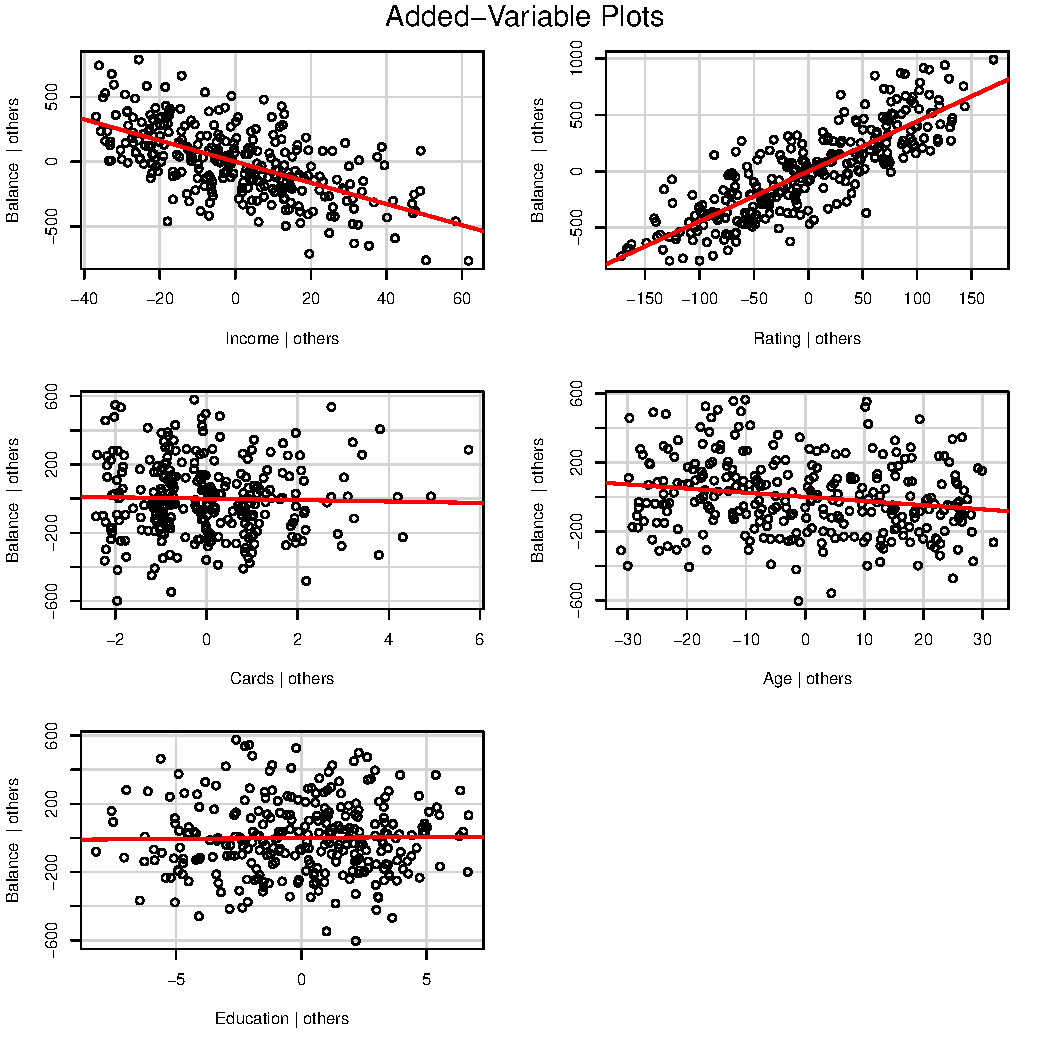
\includegraphics[width=\linewidth]{AVPlot.pdf}
\caption{Added variable plots}
\label{AV}
\end{minipage}\hfill
\begin{minipage}[t]{.45\linewidth}
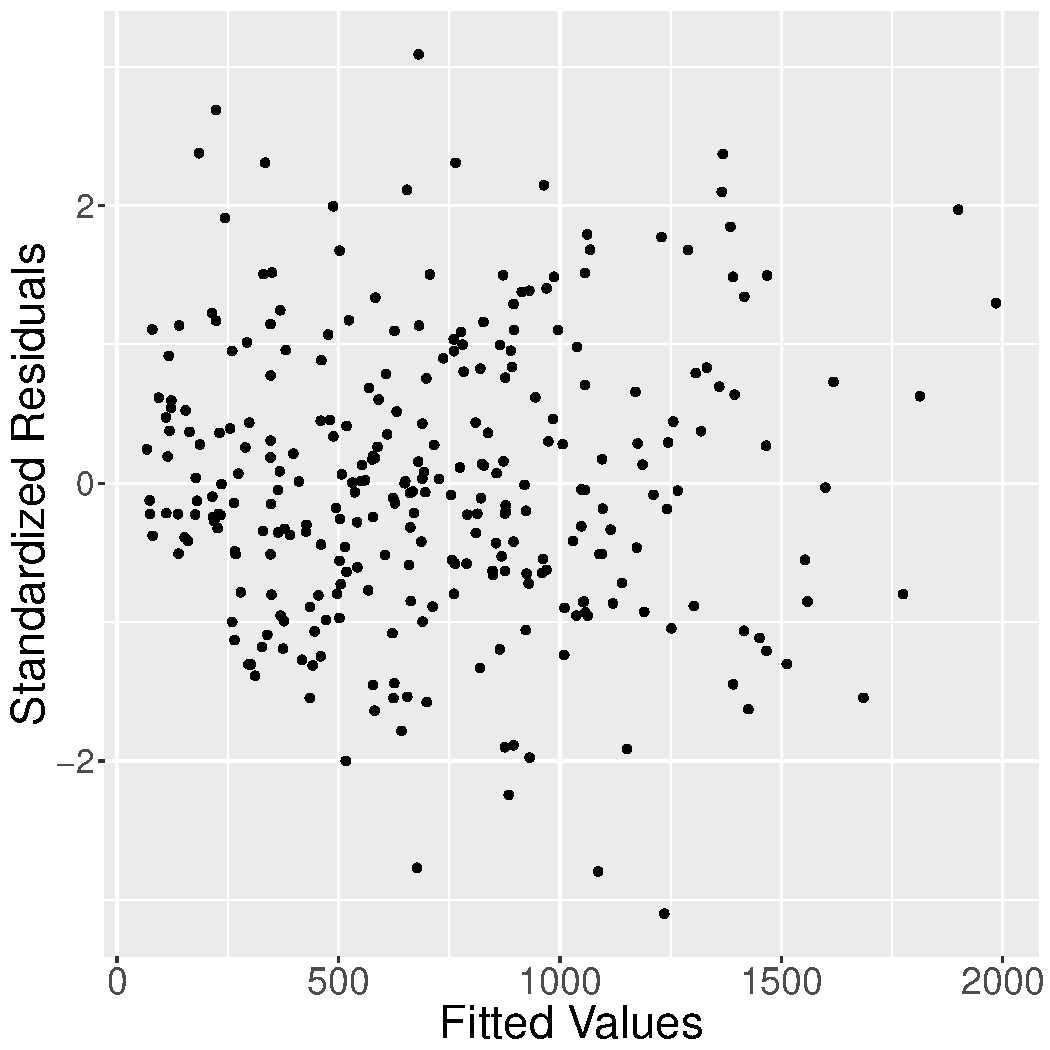
\includegraphics[width=\linewidth]{fitted.pdf}
\caption{Residuals vs. Fitted Values}
\label{fitted}
\end{minipage}
\end{figure}

\begin{figure}
\centering
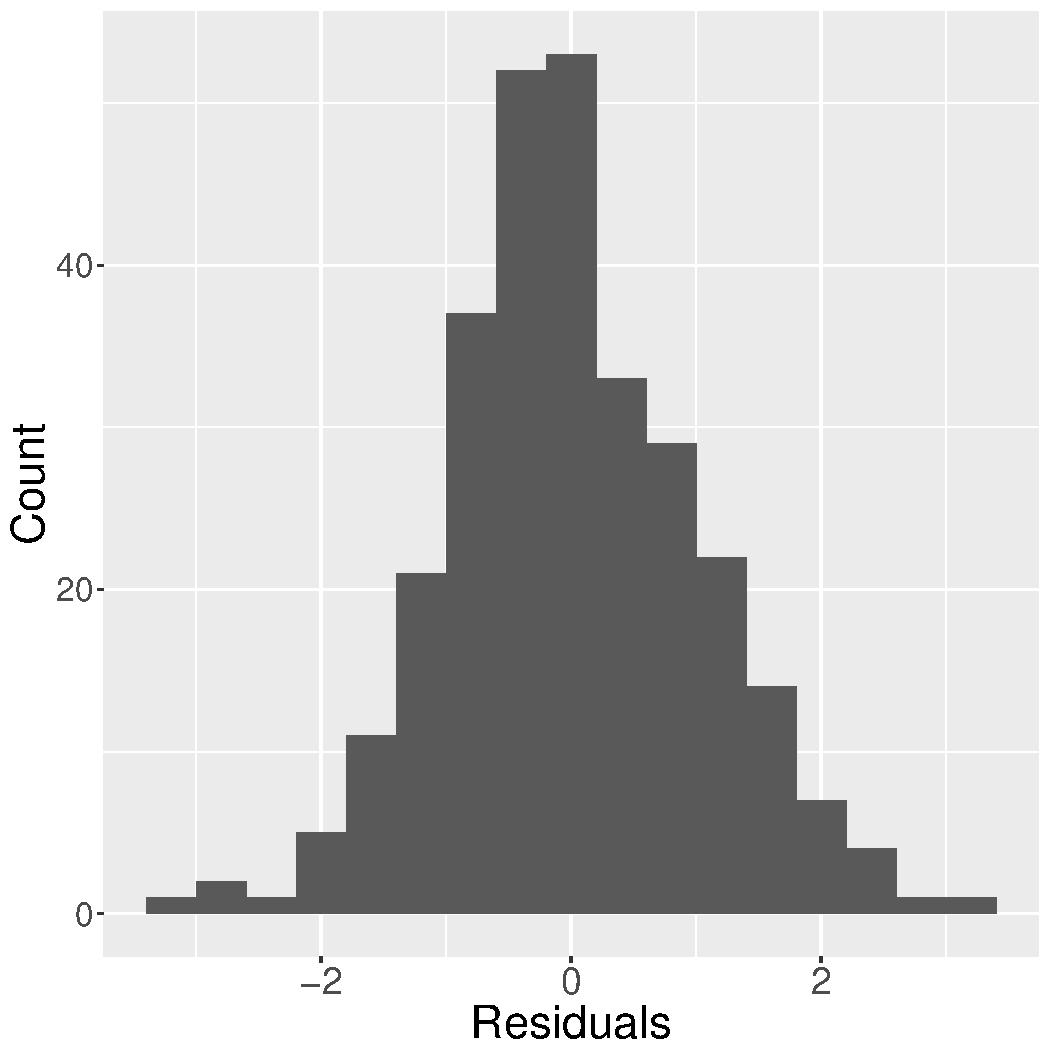
\includegraphics[width = 5.5cm]{resids.pdf}
\caption{Standardized residuals of uncorrelated model}
\label{resids}
\end{figure}

In addition to the tests above we used cross validation to calculate the root mean squared error (RMSE) and the coverage of the $95\%$ prediction interval. To preserve the time series while cross validating we fit the first 38 data points (this was the number needed to fully train the model through both summer and winter seasons with both solar and non solar data points) and then predicted the $39^{th}$ data point. We then trained on the first 39 points and predicted the $40^{th}$ data point. The process was repeated 12 times until all of the remaining data points were predicted. We calculated an RMSE of $\$27.07$ meaning that on average our predictions were $\$27.07$ off of the true values. We also found that the coverage of our 95$\%$ prediction intervals was $83\%$. While this is lower than expected the only two data points not covered were January and February 2018. Examination of Figure \ref{fig:billsummary} shows that these two months are quiet a bit higher than any other month with solar installed. We would expect that with more data that the coverage of the prediction interval would improve. 

 
\section{Results}

To show how much money is saved on average monthly, we can create a contrast matrix to contrast the difference paid without solar over a calendar year (which accounts for a fourth of the months being in summer and winter) minus the amount spent on a year with solar. This produces a monthly savings estimate of \$85.89 in monthly savings, with a 99\% confidence interval of (\$66.90, \$104.89).

\begin{figure}
\centering
\includegraphics[width = 8cm]{amount_saved.pdf}
\caption{Savings Over Time}
\label{fig:savings}
\end{figure}

The amount saved over time is shown in Figure \ref{fig:savings}. The wiggliness shows that the savings are high during the summer and small during the winter. We expect this homeowner to have saved $\$8000$ by Noveber 2023 with an interval between May 2023 and November 2024 (see Figure \ref{fig:savings}). To create this prediction interval we took the quantiles of the the distribution of the predicted differences ($p_i$) where,

\begin{equation*}
p_i \sim N(x^*_i\beta, x^*_i(X^TR^{-1}X)^{-1}x^{*T}_i + 2i\sigma^2)
\end{equation*}

Where $x^*_i$ is the design matrix for the difference in costs in the $i^{th}$ month after solar panels were installed, X is the design matrix for original data, R is the variance covariance structure, and $\sigma^2$ is the variance of residuals. The $2i\sigma^2$ accounts for increasing variance as more predictions are made. To account for the differences within the range of the data we simply subtracted the predicted non-solar costs from the actual costs with the solar panels installed. 
This means it will take anywhere from 86-102 months for this homeowner to recoup the cost of buying and installing solar panels. 






\section{Conclusion}
By fitting an AR(1) model we were able to estimate (1) the average amount that solar panels reduce power bills  and (2) the expected amount of time it will take the homeowner to recoup the $\$8000$ spent to purchase and install the solar panels. 

Our approach had several shortcomings. As noted before, our errors had heavier tails than normally distributed data. Additionally, predicting forward into the future involves a lot of extrapolation, which could easily be inaccurate due to price change, technological change, or even climate change. In addition, several approximations were made when assessing predictive uncertainty, and a Bayesian model would likely have captured the uncertainty better. Future work  could add additional data such as weather and price data as covariates and might allow for more precise savings estimates.

\end{document}
